\documentclass{report}
\usepackage[a4paper, margin=1in]{geometry}

\usepackage[utf8]{inputenc}
\usepackage[francais]{babel}
\usepackage[hidelinks]{hyperref}
\usepackage{graphicx}

\title{CPA - Graphes de terrain}
\author{Basile Pesin\\Sorbonne Université}

\begin{document}
\maketitle

\chapter{Introduction aux graphes de terrain (TME3)}

\section{To get things started}

\subsection*{Cleaning data}
Pour nettoyer (en particulier le graphe des emails) on commence par classer sur chaque ligne le plus petit numéro suivi du plus grand, grace au programme décrit dans \textit{inner-sort.c}. On classe ensuite chaque ligne et supprime les doublons avec la commande \textbf{sort -n -t " " -k1,1 -k2,2 -u email-Eu-core.txt -o email-Eu-core.out.txt}.

\subsection*{Size of the graph}
Les taille des graphes (que ce soit en nombre de noeuds ou d'arètes) sont bien conformes à celles données sur \url{https://snap.stanford.edu/}. On constate une petite différence en terme de nonmbre de noeuds, qui est du au fait qu'on prend en compte les noeuds n'apparaissant dans aucune arète (on se base sur l'identifiant du noeud) contrairement aux chiffres donnés par Stanford.

\subsection*{A special quantity}
On trouvera dans le centerau suivant les quantités $Q_g$ et les temps d'exécutions $T_g$ pour les cinq graphes proposés.

\begin{center}
  \begin{tabular}{|l|l|l|}
    \hline
    G & $Q_g$ & $T_g$ \\
    \hline
    email-EU-core & 94487825 & 9ms\\
    Amazon & 103415531 & 426ms \\
    LiveJournal & 789000450609 & 14s \\
    Orkut & 22292678512329 & 47s \\
    Friendster & 379856554324947 & 15min \\
    \hline
  \end{tabular}
\end{center}
On constate que le temps d'exécution pour le graphe de friendster est très important. Dans certaines des questions suivantes, on ne traitera pas ce graphe (par manque de temps).

\subsection*{Degree distribution}
On trouvera ci-dessous les distributions de degrés pour les cinq graphes proposés.
\begin{center}
  \includegraphics[height=.3\paperwidth]{assets/email-EU-core-dist.png}
  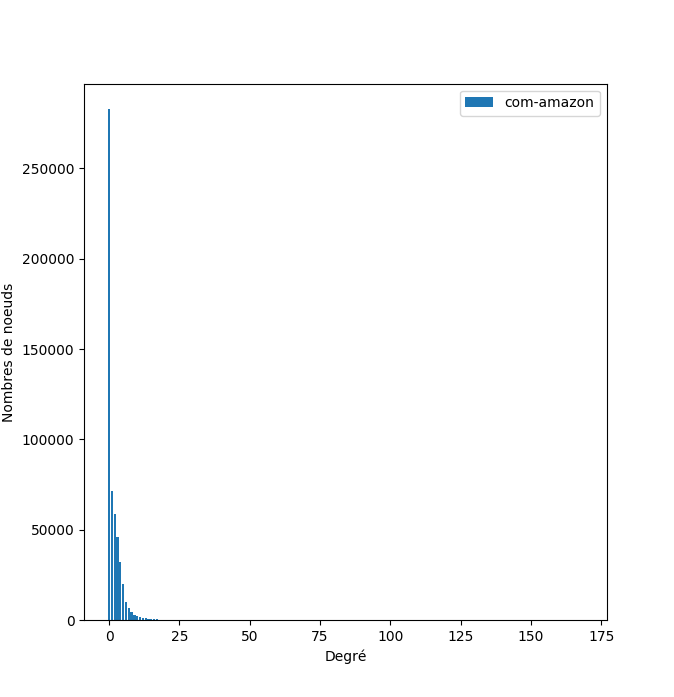
\includegraphics[height=.3\paperwidth]{assets/com-amazon-dist.png}
  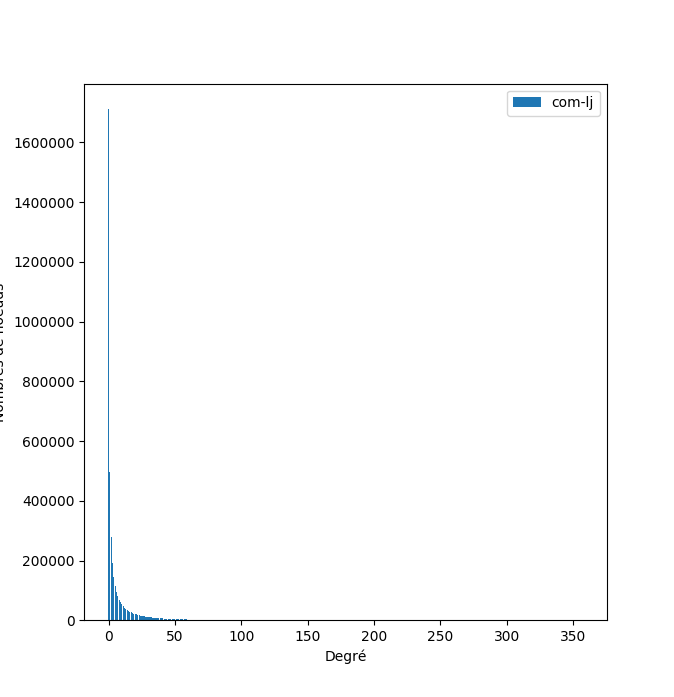
\includegraphics[height=.3\paperwidth]{assets/com-lj-dist.png}
  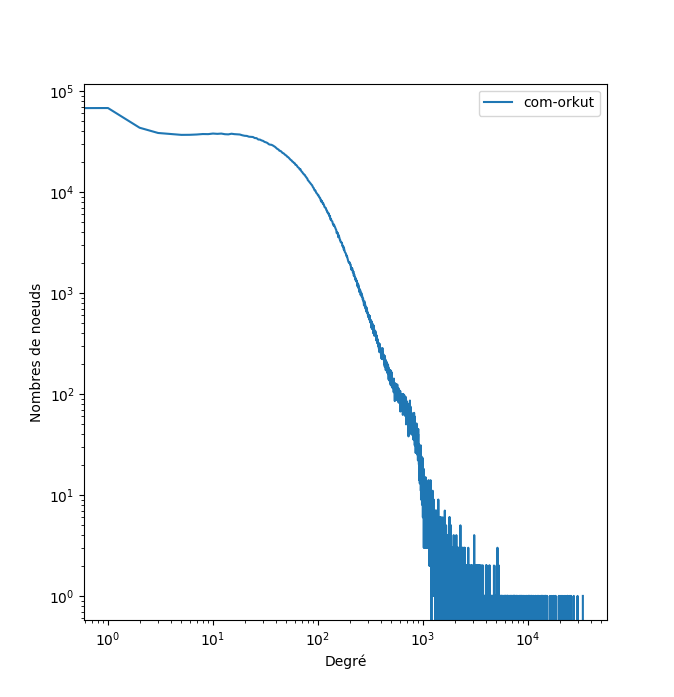
\includegraphics[height=.3\paperwidth]{assets/com-orkut-dist.png}\\
\end{center}
On constate qu'il y a énormément de noeuds avec un degré très faible, et très peu avec un fort degré (ce qui était une propriété predictible des graphes de terrains).

\section{Load a graph in memory}
On trouvera ci-dessous la taille en mémoire mesurée pour les trois structures de données et les cinq graphes proposés.

\begin{center}
  \begin{tabular}{|l|l|l|l|}
    \hline
    G & egde list & adjacency matrix & adjacency array \\
    \hline
    email-EU-core & 133ko & 4Mo & 70ko \\
    Amazon & 7Mo & Trop & 5Mo \\
    LiveJournal & 270Mo & Trop & 154Mo \\
    Orkut & 1Go & Trop & 500Mo \\
    Friendster & Trop & Trop & Trop \\
    \hline
  \end{tabular}
\end{center}
On constate très vite que la structure matrice d'adjacence est impraticable pour de tels graphes, puisque sa taille croit quadratiquement par rapport au nombre de noeuds du graphes (on peut calculer par exemple que pour le graphe Amazon, le plus petit de nos grands graphes, sa taille serait de $n^2 \times sizeof(int)$, soit sur mon architecture $334863^2 \times 4 \simeq 450Go$). Pour ce qui est des autres structures de données, on constate que le centerau d'adjacence est un peu plus efficace que la liste d'aretes (d'un facteur 2). Etant donné que cette structure propose aussi une meilleure efficacité pour beaucoup de problèmes, on aura tendance à la préférer dans la suite, sauf cas particulier.\\
Dans le cas particulier du graphe de Friendster, le graphe est trop grand pour tenir dans la RAM de mon ordinateur porcenter, quelque soit la structure de données utilisée. On note que la taille thèorique de l'adjacency array pour ce graphe serait de l'ordre de $2\times m \times sizeof(unsigned\,int)$ soit sur mon architecture $2 \times 1806067135 \times 4 \simeq 14.5Go$. Cela nous fait une raison de plus pour ignorer ce graphe dans les prochaines questions.

\section{Breadth-first search and diameter}

La fraction des nodes dans la plus grand composante connectée est bien celle qu'on s'attendait à trouver, à savoir:
\begin{center}
  \begin{tabular}{|l|l|}
    \hline
    G & node dans la WCC \\
    \hline
    email-EU-core & 0.981\\
    Amazon & 1.000\\
    LiveJournal & 1.000\\
    Orkut & 1.000\\
    \hline
  \end{tabular}
\end{center}

Pour ce qui est des diametres, on a tendance à trouver des bornes inférieures un peu plus grandes que celles prévues sur \url{https://snap.stanford.edu}, à savoir:
\begin{center}
  \begin{tabular}{|l|l|}
    \hline
    G & borne inf du diametre \\
    \hline
    email-EU-core & 7\\
    Amazon & 48\\
    LiveJournal & 22\\
    Orkut & 10\\
    \hline
  \end{tabular}
\end{center}

\section{Listing triangles}
On prends seulement en compte dans le temps d'exécution la partie calcul de triangles proprement dite, et pas le chargement du graphe. On trouve alors les nombres de triangles et les temps de calcul suivants:\\
\begin{center}
  \begin{tabular}{|l|l|l|l|l|}
    \hline
    G & nombre de triangles & temps d'exécutation & transitivity & clustering\\
    \hline
    email-EU-core & 105461 & 68ms & 0.128 & 0.310\\
    Amazon & 667129 & 635ms & 0.094 & 0.276\\
    LiveJournal & 177820130 & 200s & 0.032 & 0.22\\
    Orkut & 627584181 & 28min & 0.0145 & 0.125920\\
    \hline
  \end{tabular}
\end{center}

\chapter{Detection de communautés (TME4)}

\section{Simple benchmark}

\begin{center}
  \begin{figure}[!h]
    \centering
    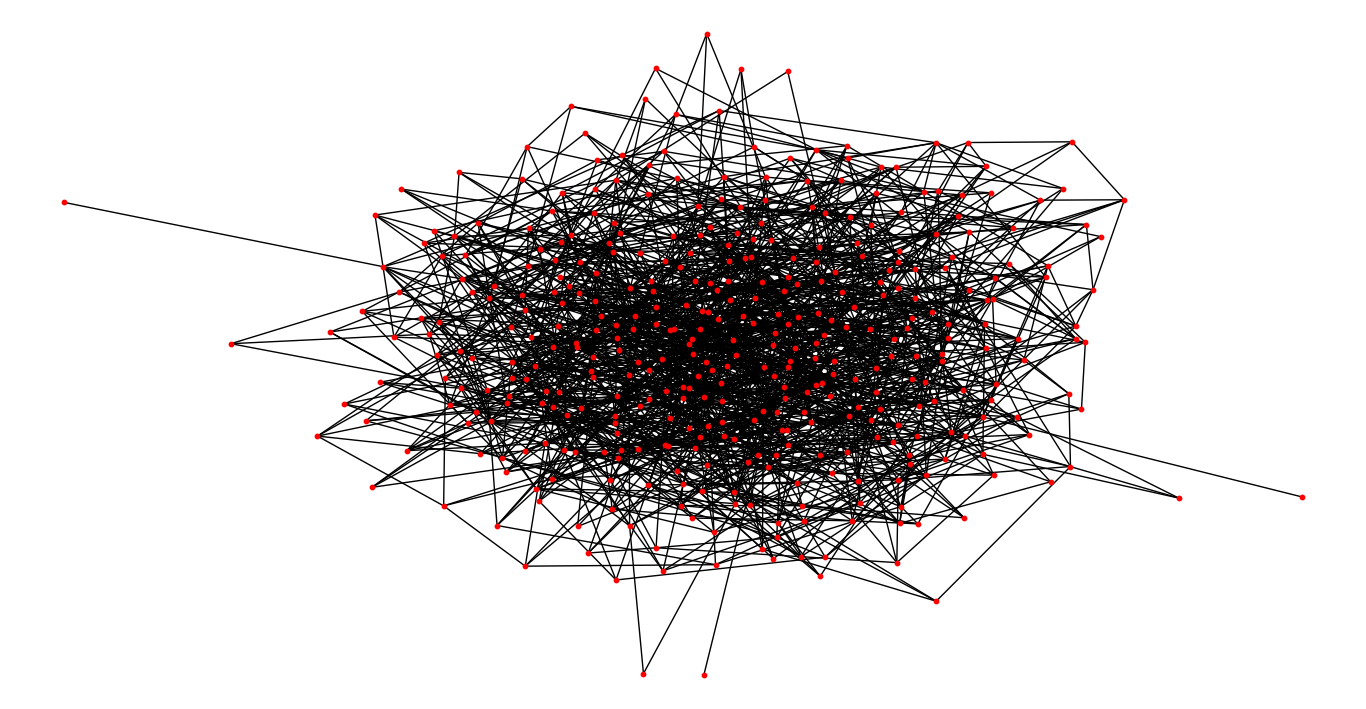
\includegraphics[width=0.3\paperwidth]{assets/0101.png}\\
    \caption*{$p=0.01, q=0.01$}
  \end{figure}
  \begin{figure}[!h]
    \centering
    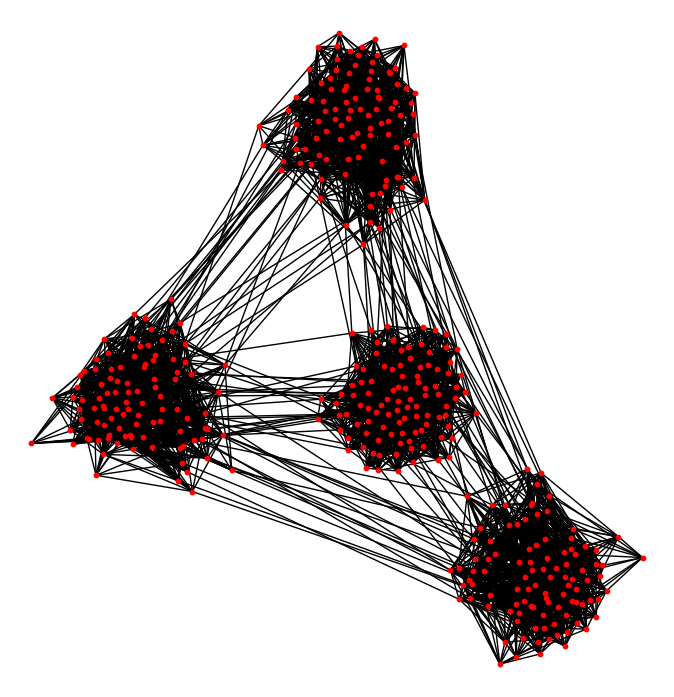
\includegraphics[width=0.3\paperwidth]{assets/01001.png}\\
    \caption*{$p=0.01, q=0.001$}
  \end{figure}
  \begin{figure}[!h]
    \centering
    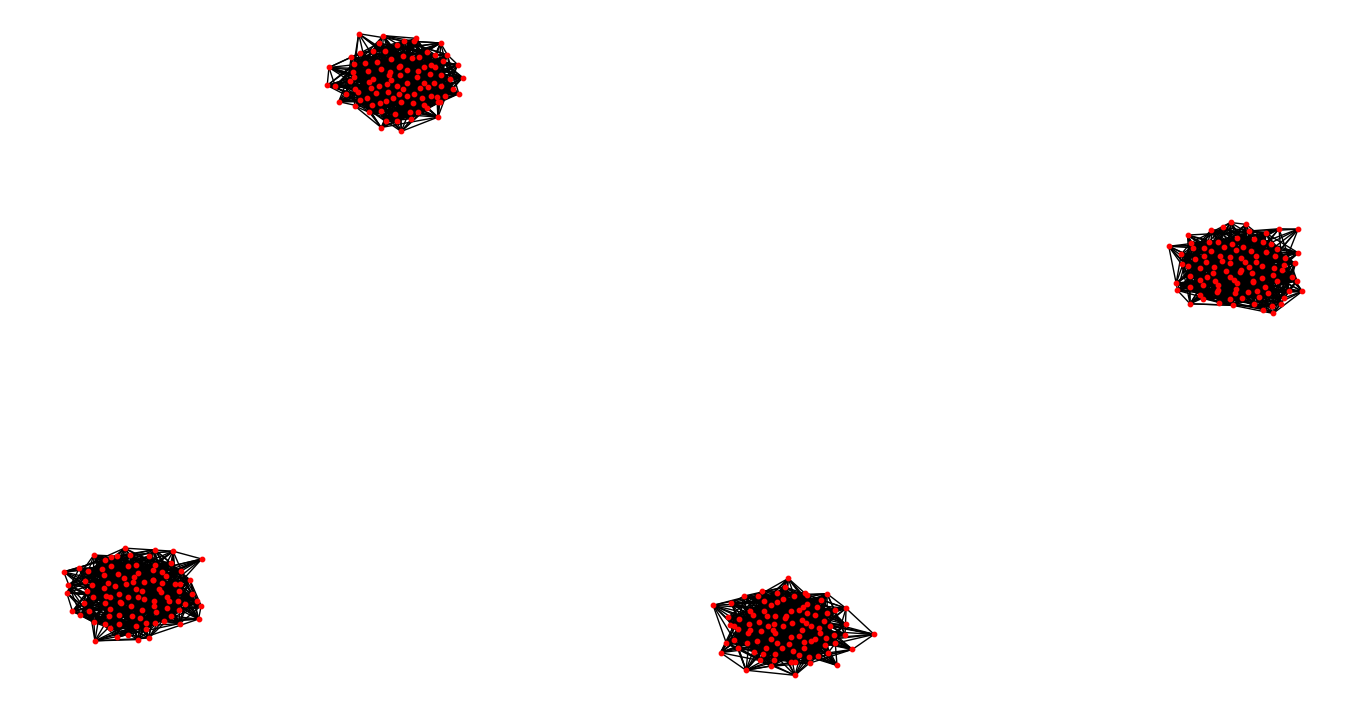
\includegraphics[width=0.3\paperwidth]{assets/01000001.png}\\
    \caption*{$p=0.1, q=10^-6$}
  \end{figure}
\end{center}

On se rends aisément compte que plus le ration $p/q$ augmente, plus les communautés sont éloignées les unes des autres mais fortement connectée en interne. On peut alors s'attendre à ce qu'une communauté avec un ration $p/q$ élevé (telle que la troisième représentée ci-contre) soit plus facile à detecter.

\section{Label propagation}
En reprenant les graphes précédants:

\begin{center}
  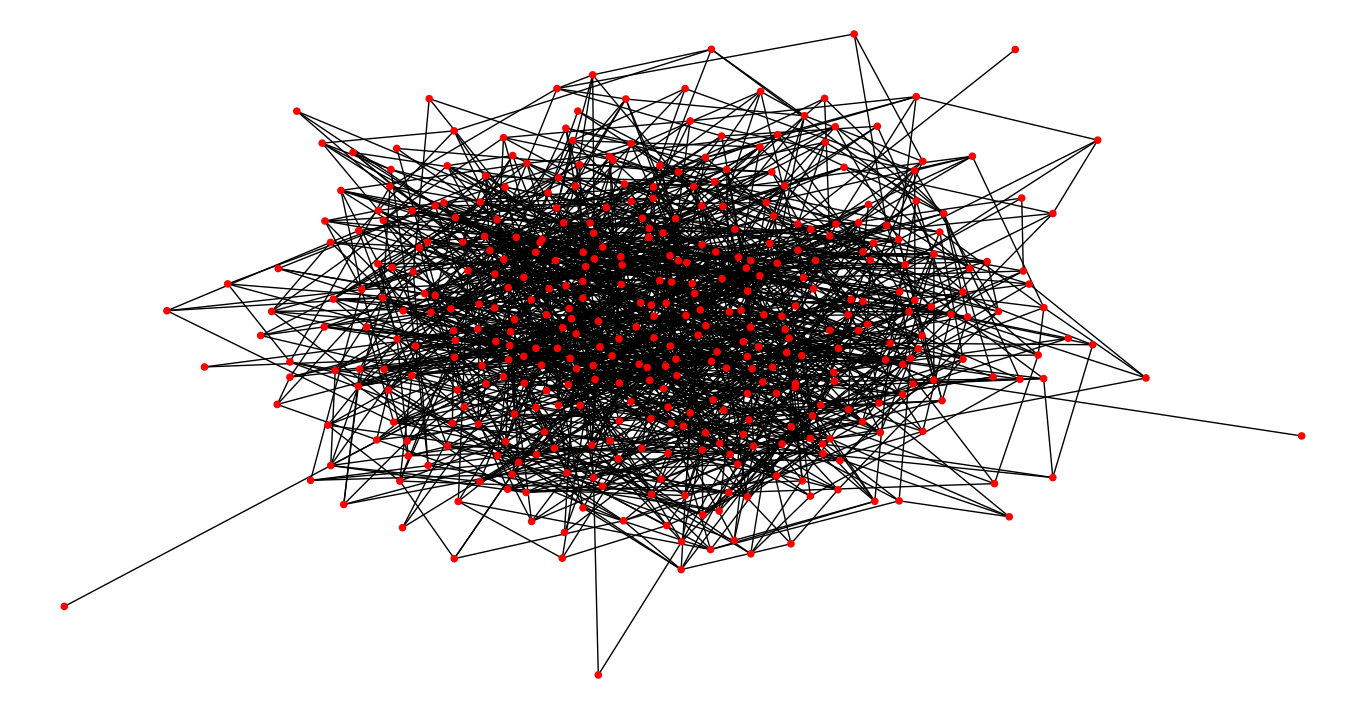
\includegraphics[width=0.3\paperwidth]{assets/0101coms.png}\\
  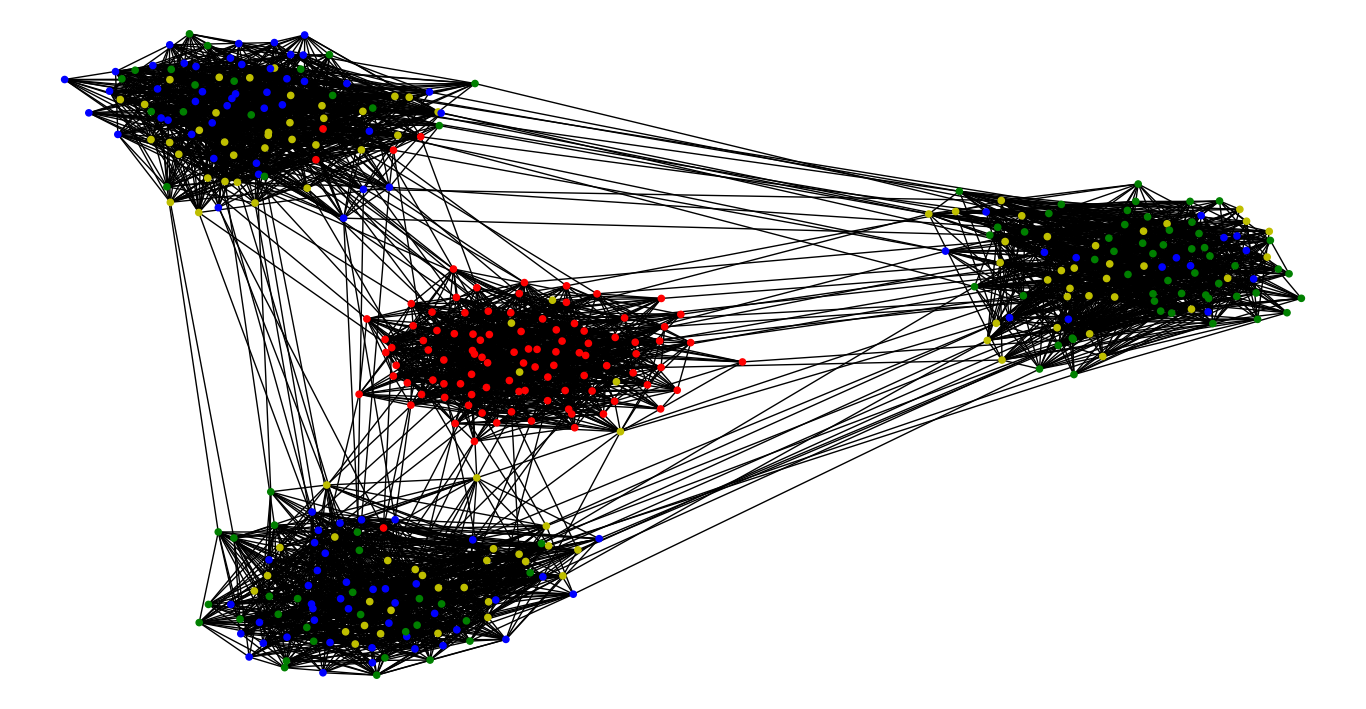
\includegraphics[width=0.3\paperwidth]{assets/01001coms.png}\\
  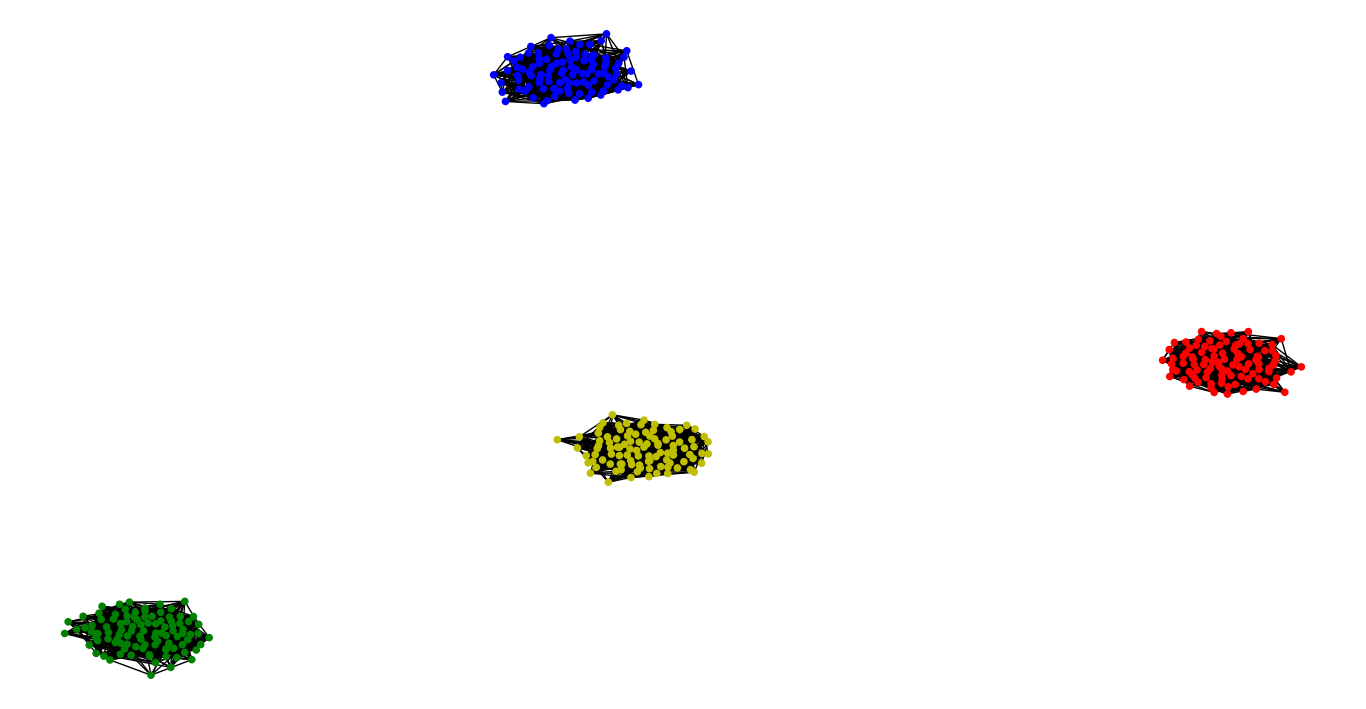
\includegraphics[width=0.3\paperwidth]{assets/01000001coms.png}\\
\end{center}

On remarque que même si l'algorithme de propagation de labels est plutôt efficace pour les cas ``triviaux'' 1 et 3, il présente quelques difficultés pour correctement délimiter les communautés du deuxième exemple.

\begin{center}
  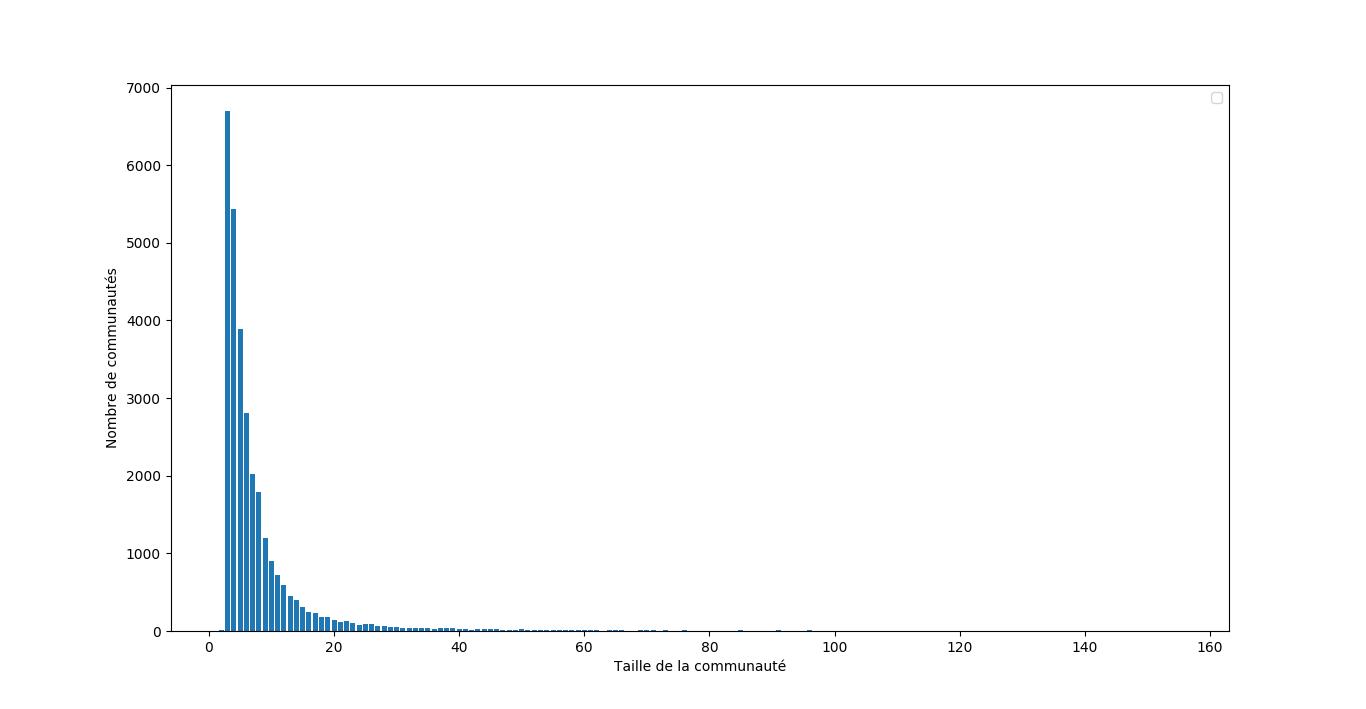
\includegraphics[width=0.6\paperwidth]{assets/histSizes.png}
\end{center}

En exécutant l'algorithme sur le graphe de youtube, on remarque que la grande majorité des graphes de terrains sont de petite taille, et que les très grandes communautés sont assez rare (encore un exemple de la loi des puissances).\\

\begin{center}
  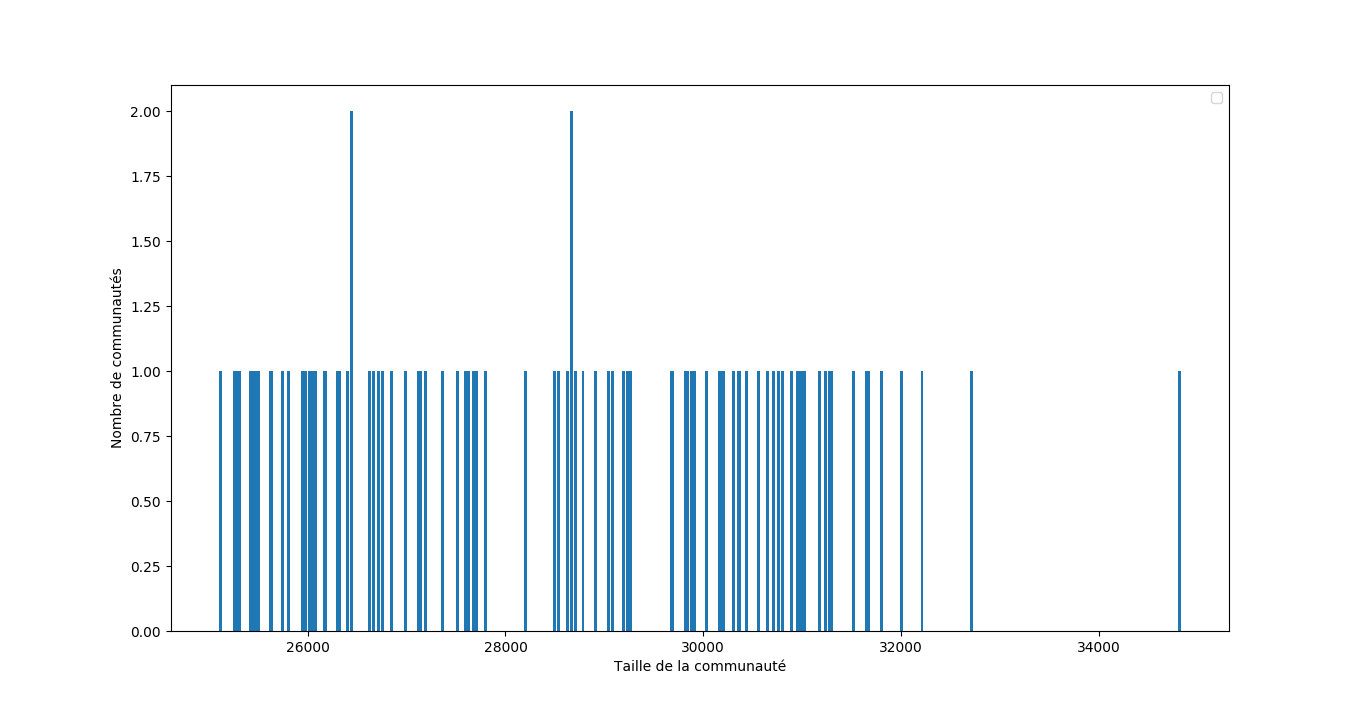
\includegraphics[width=0.6\paperwidth]{assets/nbComs.png}
\end{center}

En exécutant ce code 100 fois (pas 1000, par manque de temps principalement), on remarque que le résultat varie malgré tout (puisque l'algorithme de propagation n'est pas deterministe) entre 26000 et 34000 (soit un écart de $25\%$). Cet écart étant très important, on peut donc en conclure que cet algorithme n'est pas très efficace, puisque trop influencé par le hasard.

\section{New algorithm}
On implémente un algorithme par division, dans lequel la force d'un lien entre les noeuds $u$ et $v$ est le nombre de voisins en commun de $u$ et $v$. On répète cet algorithme en ne gardant que les liens de force supérieure à $\frac{maxForce}{10}$ (plutôt bonne valeur trouvée experimentalement en testant plusieurs valeurs), tout en mettant bien sur à jour les forces des liens au fur et à mesure. On construit ensuite les communautés par liens toujours connectés (en faisant un BFS donc).\\
L'algorithme est implémenté dans le fichier \textit{exo4.cpp}.

\begin{center}
  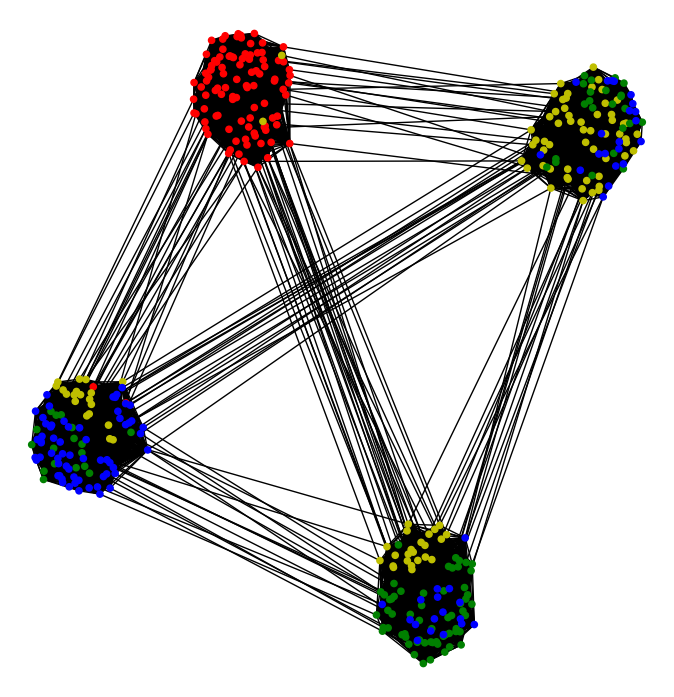
\includegraphics[width=0.6\paperwidth]{assets/exo4.png}
\end{center}

Comme on le voit dans la figure ci dessus (générée par notre benchmark de l'exercice 1 avec $p = 0.5$ et $q = 0.001$) l'algorithme fonctionne plutôt bien avec des valeurs de p et q très prononcées. C'est moins le cas si ces valeurs sont plus proches. Cela dit, cet algorithme dépend beaucoup du nombre de triangles présents dans le graphe. On peut donc se dire que dans un graphe réel, qui contiendra plus de triangles que le notre (puisque la benchmark n'a pas tendance à en générer) l'algorithme fonctionnera mieux.

\section{Validation}

On a mesuré les temps d'exécution au moyen de la command $time$, ce qui signifie que les temps mesurés prennent en compte le temps d'ouverture et de lecture du graphe. Etant donné que le programme $louvain$ prends en entrée un fichier binaire déjà optimisé, on peut s'attendre à ce que les résultats soient un peu faussés en faveur de Louvain.

\begin{center}
  \begin{tabular}{|l|l|l|l|}
    \hline
    Algorithme & Label Propagation & Louvain & Mon algorithme\\
    \hline
    Benchmark (n = 10000) & 0.45s & 0.05s & 5.03s\\
    Amazon (n = 334863) & 4.46s & 5.11s & 30.21s\\
    Youtube (n = 1134890) & 17s & 11.06s & 7min\\
    \hline
  \end{tabular}
\end{center}

On constate que l'algorithme réalisé ne passe pas bien à l'echelle (cela est principalement du aux bfs nécessaires pour reformer les communautés à la fin de l'algorithme). On pourrait améliorer cet algorithme en utilisant une structure de donnée union-find.

\chapter{PageRank (TME5)}

\section{PageRank (directed graph)}

Les 5 pages avec le plus haut PageRank du graphe (par PageRank décroissant) sont:

\begin{center}
  \begin{tabular}{|l|l|l|}
    \hline
    Rang & Page & PageRank\\
    \hline
    $1$ & United States & $3.64\mathrm{e}{-3}$\\
    $2$ & United Kingdom & $1.59\mathrm{e}{-3}$\\
    $3$ & Germany & $1.36\mathrm{e}{-3}$\\
    $4$ & 2007 & $1.36\mathrm{e}{-3}$\\
    $5$ & 2006 & $1.26\mathrm{e}{-3}$\\
    \hline
  \end{tabular}
\end{center}

D'autre part, les pages avec les rangs les plus faibles (par PageRank croissant) sont:

\begin{center}
  \begin{tabular}{|l|l|l|}
    \hline
    Rang & Page & PageRank\\
    \hline
    $n$ & I Have Dreamed & $7.31\mathrm{e}{-8}$\\
    $n-1$ & I Have Dreamed (album) & $7.31\mathrm{e}{-8}$\\
    $n-2$ & The Other Side of Life (Sound Pollution and Rotting Christ split album) & $7.31\mathrm{e}{-8}$\\
    $n-3$ & History of Bayern Munich & $7.31\mathrm{e}{-8}$\\
    $n-4$ & Marguerite Jeanne Carpentier & $7.31\mathrm{e}{-8}$\\
    \hline
  \end{tabular}
\end{center}
On remarque que les ``flops 5'' ont tous le même score, et le classement dépend donc surtout de l'algorithme de tri utilisé.

On a obtenu ces résultats avec 20 itérations du PageRank, et on constate qu'augmenter le nombre d'itérations ne change pas les résultats, 20 semble donc être une bonne valeur.

\section{Correlations}

La loi des puissances présentes dans ces graphes fait qu'il est plus intéressants d'utiliser des echelles logarithmiques, c'est donc ce qu'on fera dans les graphiques suivants.

\begin{center}
  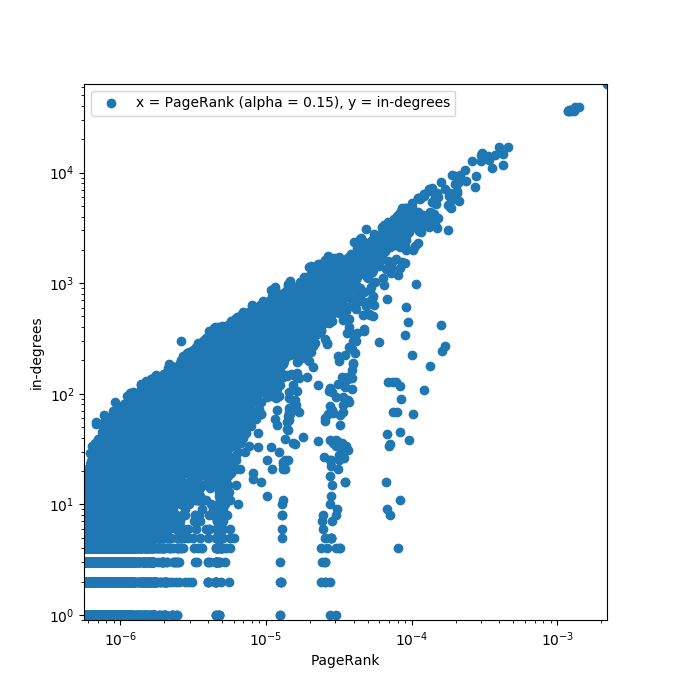
\includegraphics[width=0.25\paperwidth]{assets/pagerankindegs.png}
  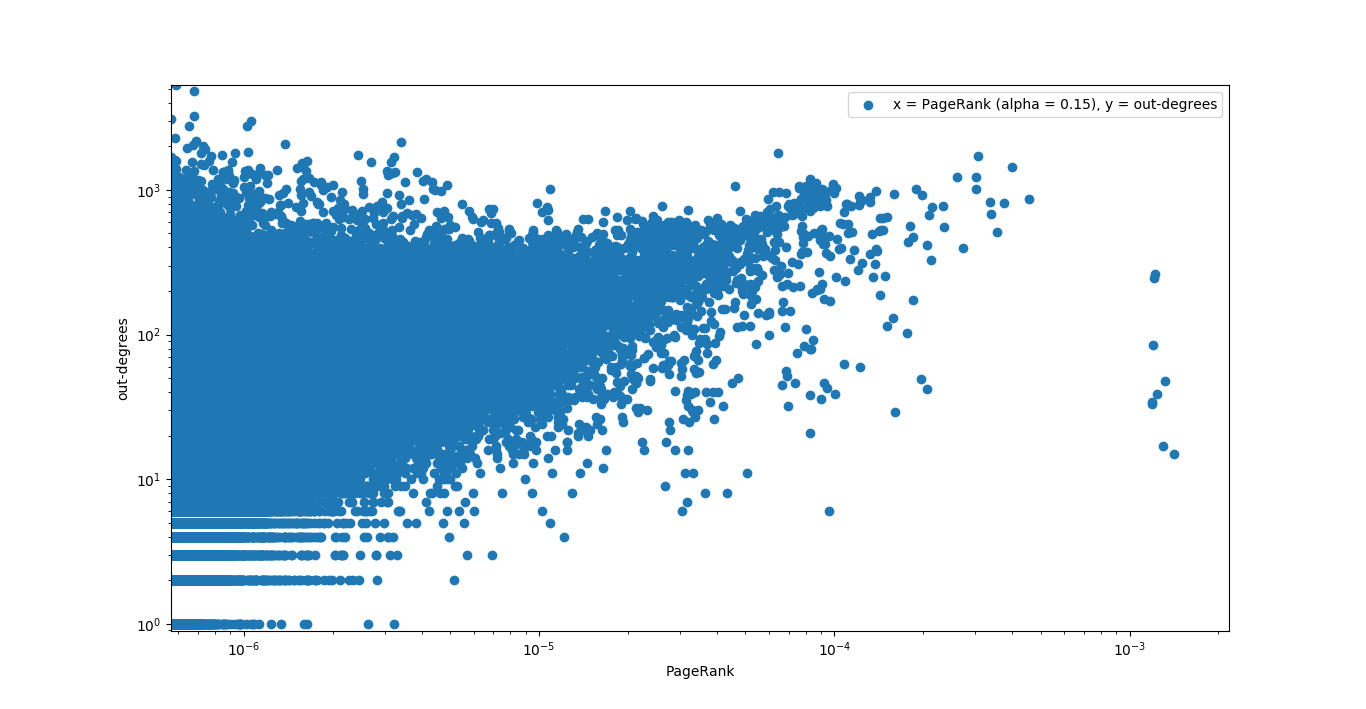
\includegraphics[width=0.25\paperwidth]{assets/pagerankoutdegs.png}
\end{center}

On remarque que dans le cas des degrés sortants, on a bien une corrélation très forte, ce qui est logique. On remarque cependant que le PageRank n'est pas non plus exactement proportionnel au degré (et heureusement, sinon on se serait embete à faire tout ça alors qu'on aurait pu simplement calculer les degrés).\\
Dans le cas des degrés sortants en revanche, il n'y a quasiment aucune corrélation.

\begin{center}
  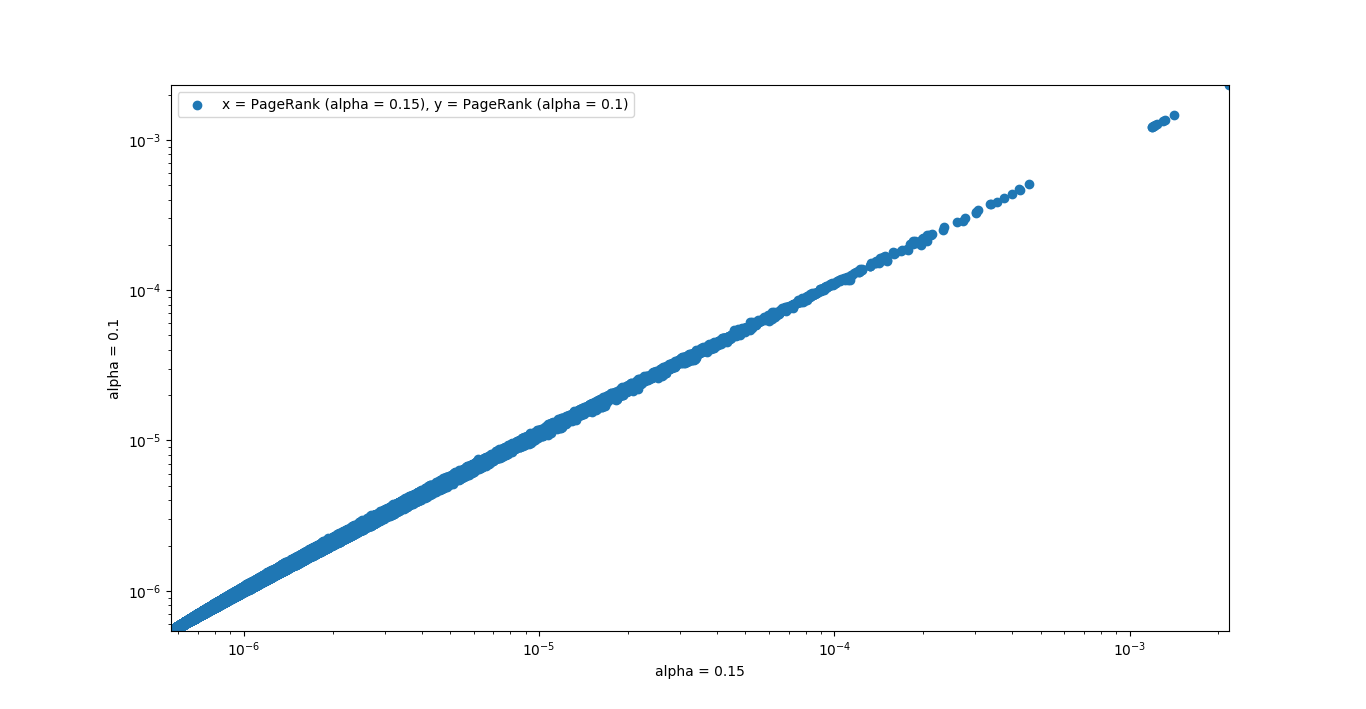
\includegraphics[width=0.25\paperwidth]{assets/pagerank01.png}
  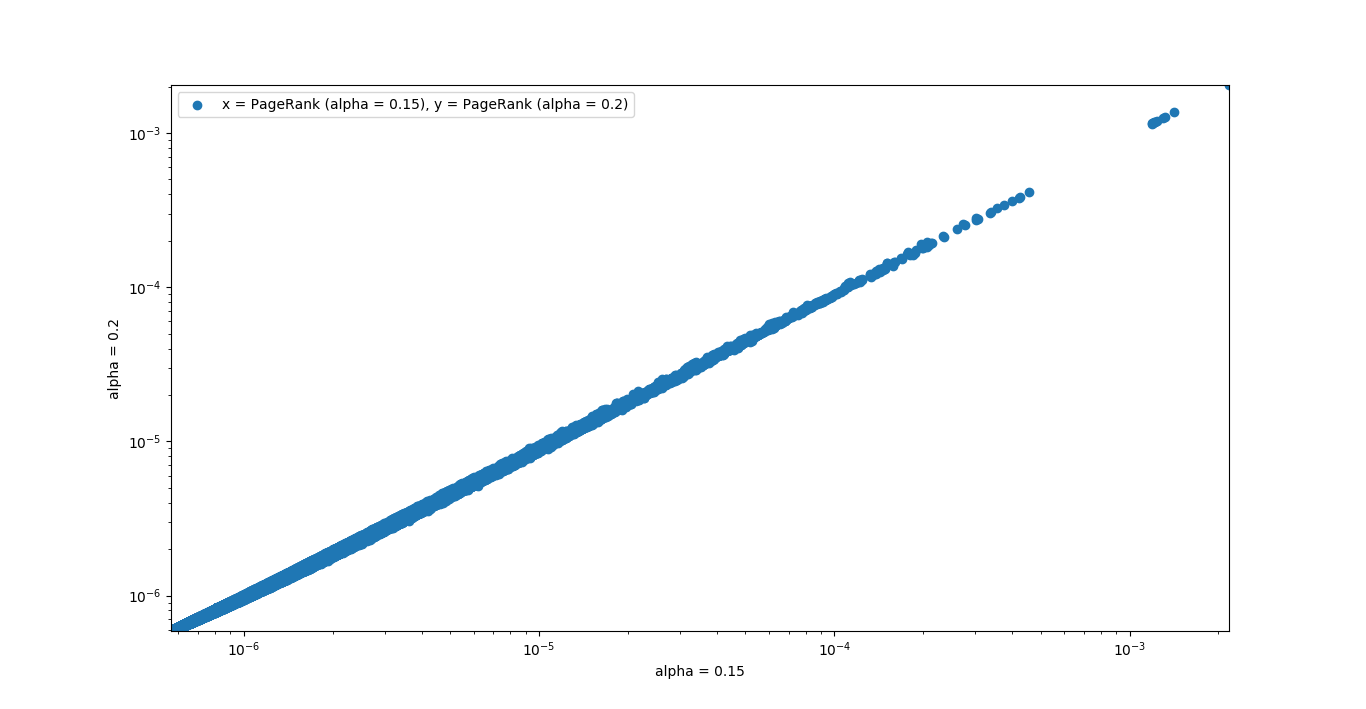
\includegraphics[width=0.25\paperwidth]{assets/pagerank02.png}
  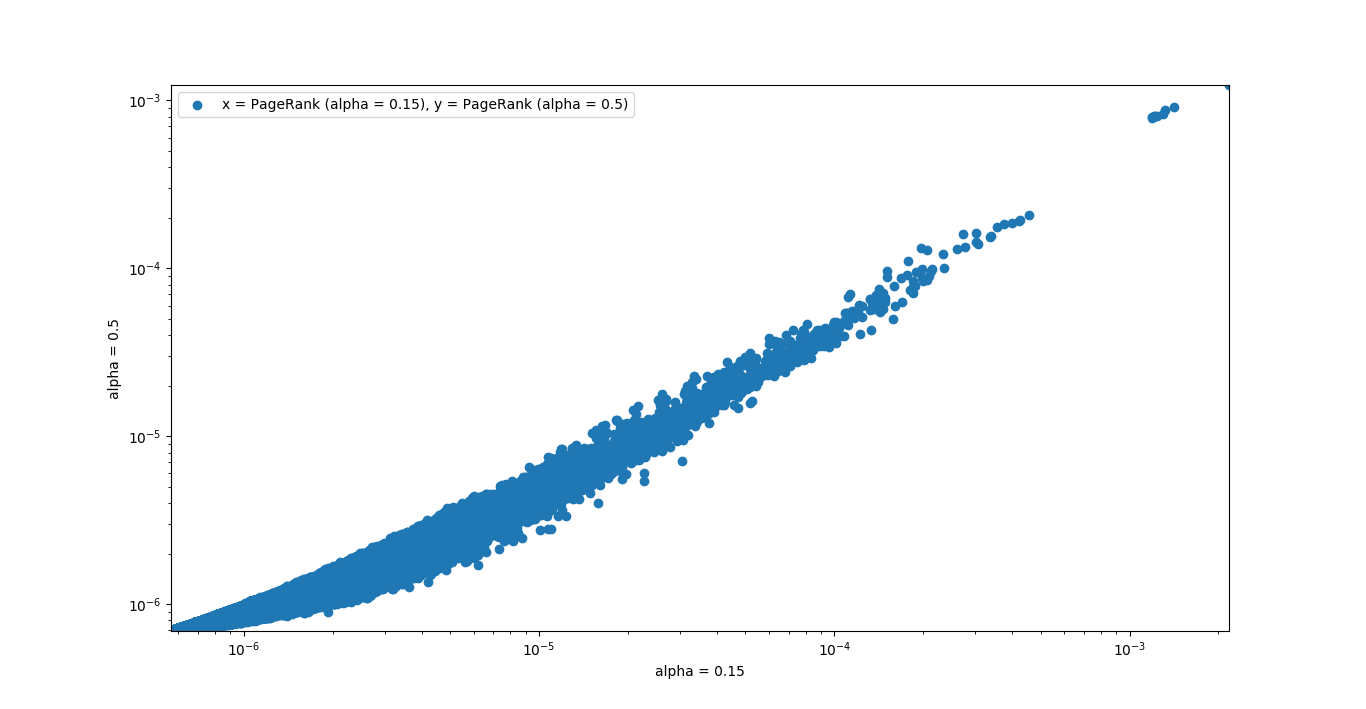
\includegraphics[width=0.25\paperwidth]{assets/pagerank05.png}
  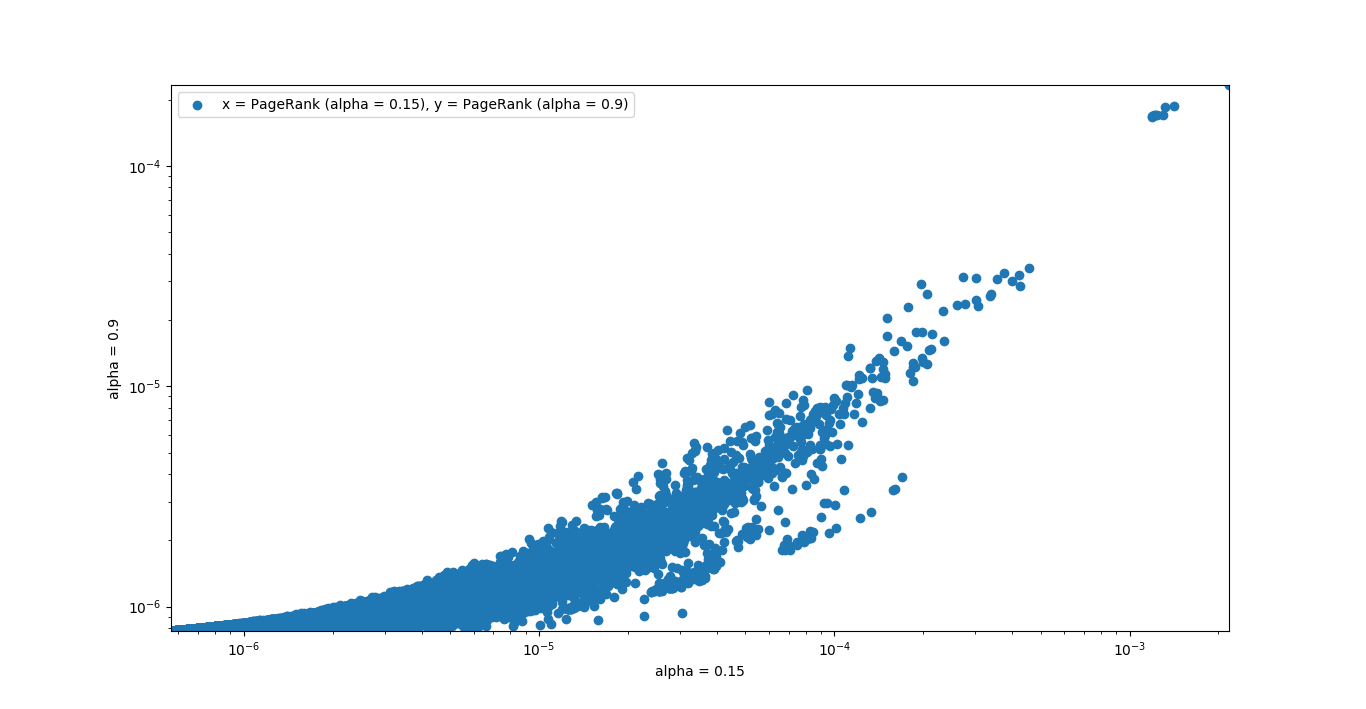
\includegraphics[width=0.25\paperwidth]{assets/pagerank09.png}
\end{center}

Comme on pouvait s'y attendre, la corrélation est forte pour des valeurs de alpha proches (et raisonnables) mais s'écroute quand alpha devient trop grand.

\section{PageRank ``sans mémoire''}
On a implémenté la version du PageRank utilisant moins de mêmoire (mais devant relire le fichier à chaque itération) dans le fichier \textit{pageranknonmem.cpp}. On a comparé les temps d'exécutions pour 20 itérations pour les 2 graphes ci-dessous:
\begin{center}
  \begin{tabular}{|l|l|l|l|}
    \hline
    Graphe & n & m & temps\\
    \hline
    Wikipédia (ss-ensemble) & 2 millions & 11 millions & 18min\\
    \href{http://konect.uni-koblenz.de/networks/wikipedia_link_en}{Wikipedia} & 12 millions & 378 millions & 2h10min\\
    \hline
  \end{tabular}
\end{center}
Malheureusement, par souci de temps, on n'a pas pu réaliser les calculs sur le graphe de Twitter (MPI) qui possède presque 2milliards de noeuds. On peut extrapoler que les calculs auraient duré au moins 10h, et malheureusement je peux rarement laisser mon PC occupé aussi longtemps sans en avoir besoin.

\section{Personnalized PageRank}
On a aussi implémenté (dans le fichier \textit{perspagerank.cpp}) le Personnalized PageRank. On le teste en Rooted PageRank avec comme point de départ la page wikipédia de la France, et $alpha = 0.2$. On obtient alors les résultats suivants:

\begin{center}
  \begin{tabular}{|l|l|}
    \hline
    Rang & Page\\
    \hline
    $1$ & France\\
    $2$ & United States\\
    $3$ & United Kingdom\\
    $4$ & Paris\\
    $5$ & Germany\\
    \hline
  \end{tabular}
\end{center}

On remarque que les Etats Unis font leur retour, cette fois ci en deuxième position derrière notre point de départ. Les autres résultats sont assez cohérents, puisque directement l'Angleterre et l'Allemagne, en plus d'avoir un pagerank important (comme on l'a vu dans l'exercice 1) sont voisins de la France.

\chapter{Densest Subgraph (TME6)}

\section{k-core decomposition}

On a calculé au moyen de la k-core decomposition la core value des 4-graphes suivants, ainsi que l'average degree density, l'average edge density et la taille des densest subgraph de chaque graphe.
\begin{center}
  \begin{tabular}{|l|l|l|l|l|}
    \hline
    G & core value & avg degree density & avg edge density & size\\
    \hline
    email-EU-core & 34 & 27.6 & 0.24 & 228\\
    Amazon & 6 & 3.9 & 0.87 & 10\\
    LiveJournal & 360 & 191 & 0.99 & 386\\
    Orkut & 253 & 227.9 & 0.02 & 25891 \\
    \hline
  \end{tabular}
\end{center}

\section{Graph mining with k-core}

En tracant la coreness des noeuds du graphes google-scholar par rapport a leur degré, on obtient le graphe suivant:
\begin{center}
  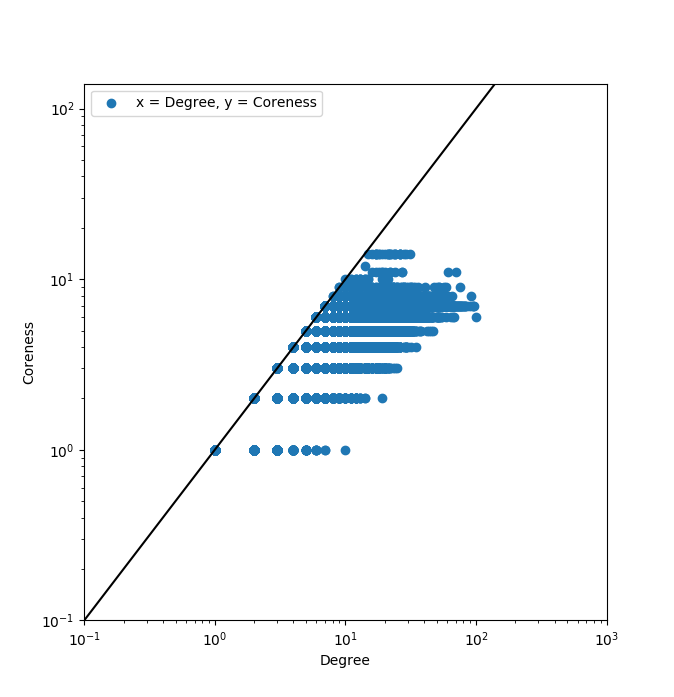
\includegraphics[height=.30\paperwidth]{assets/scholardegreecoreness.png}
\end{center}

Les points étranges sont ceux ayant une coreness très forte (proche de 14). En se référant au nom des auteurs, on découvre qu'il s'agit d'un ensemble d'auteurs travaillant au Korea Institute of Science and Technology Information (KISTI). On peut donc en déduire que ces auteurs travaillent beaucoup en collaboration et co-publient de nombreux articles (ce qui semble être confirmé en parcourant les pages Google Scholar de ces auteurs).

\section{Densest subgraph}
On utilise maintenant l'algorithme simple donné dans la slide 17 du cours pour chercher l'average degree density, l'average edge density et la taille des densest subgraph. On obtient alors les résultats suivants pour $t=10$:
\begin{center}
  \begin{tabular}{|l|l|l|l|l|}
    \hline
    G & highest density & avg degree density & avg edge density & size\\
    \hline
    email-EU-core & 28.8 & 27.4 & 0.21 & 253\\
    Amazon & 4.95 & 3.92 & 0.001 & 9977 \\
    LiveJournal & 197.9 & 190.9 & 0.21 & 1820 \\
    Orkut & 241.9 & 227 & 0.015 & 29608 \\
    \hline
  \end{tabular}
\end{center}

Et pour $t = 100$: (au dela de $t = 100$ les résultats semblent assez stable, on passera donc $t = 1000$ pour des raisons de temps)
\begin{center}
  \begin{tabular}{|l|l|l|l|l|}
    \hline
    G & highest density & avg degree density & avg edge density & size\\
    \hline
    email-EU-core & 27.7 & 27.6 & 0.24 & 228 \\
    Amazon & 4.82 & 4.8 & 0.1 & 96 \\
    LiveJournal & 193.7 & 193.2 & 0.38 & 1015 \\
    Orkut & 229.2 & 227 & 0.017 & 26528 \\
    \hline
  \end{tabular}
\end{center}

On remarque que cet algorithme est un peu plus efficace que le précédent pour $t = 100$: l'average degree density obtenue est un peu supérieure à celle obtenue avec l'algorithme précédant (qui était une 2-approximation). On remarque d'ailleurs que le density score est tres proche (mais toujours supérieur) a l'average degree density (ce qui est normal puisque c'est une borne supérieure).

\section{Triangle densest prefix}
On va maintenant calculer le densest prefix en fonction des triangles plutot que des aretes. Pour ce faire, on on itère sur les triangles plut que sur les aretes. Malheureusement, le nombre de triangles étant très grand, on ne peut les trocket en mémoire et on doit donc les recalculer à chaque itération. On obtient alors pour $t = 100$ les résultats suivants:
\begin{center}
  \begin{tabular}{|l|l|l|l|l|}
    \hline
    G & avg triangle density & avg edge density & size\\
    \hline
    email-EU-core & 167 & 0.27 & 203\\
    Amazon & 4.5 & 0.07 & 126\\
    LiveJournal & 13263 & 0.4 & 957\\
    Orkut & 623745 & 0.07 & 5381 \\
    \hline
  \end{tabular}
\end{center}
On remarque qu'effectivement, les densest subgraphs obtenus sont plus denses et plus petit que ceux obtenus par l'algorithme de l'exercice 3.

\end{document}
